\documentclass{standalone}
\usepackage{tikz}
\usetikzlibrary{positioning,arrows.meta}

% COLORS
\usepackage{xcolor}
\colorlet{myred}{red!80!black}
\colorlet{myblue}{blue!80!black}
\colorlet{mybluee}{myblue!80!black}
\colorlet{mygreen}{green!60!black}
\colorlet{myorange}{orange!70!red!60!black}
\colorlet{mydarkred}{red!30!black}
\colorlet{mydarkblue}{blue!40!black}
\colorlet{mydarkgreen}{green!30!black}

\begin{document}
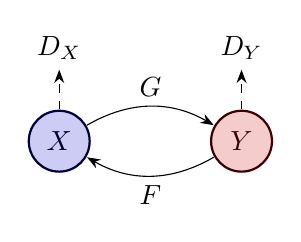
\begin{tikzpicture}[
    >=Stealth, % for default LaTeX arrow head
    box/.style={thick,circle,minimum size=22,inner sep=0.5,outer sep=0.6},
]

% Nodes
\node[blue!20!black,draw=myblue!30!black,fill=myblue!20, box] (X) {$X$};
\node[red!20!black,draw=myred!30!black,fill=myred!20, box, right=1.5cm of X] (Y) {$Y$};

% Arrows
\draw[->] (X) to[bend left=30] node[above] {$G$} (Y);
\draw[->] (Y) to[bend left=30] node[below] {$F$} (X);

% Vertical arrows
\draw[->, dashed] (X.north) -- +(0,0.5cm) node[above] {$D_X$};
\draw[->, dashed] (Y.north) -- +(0,0.5cm) node[above] {$D_Y$};

\end{tikzpicture}
\end{document}